\documentclass[11pt]{article}
\usepackage[margin=1in]{geometry}
\usepackage[T1]{fontenc}
\usepackage{lmodern,microtype,amsmath,amssymb,amsthm,booktabs,graphicx}
\usepackage[hidelinks]{hyperref}
\newtheorem{theorem}{Theorem}[section]
\newtheorem{proposition}[theorem]{Proposition}
\newtheorem{lemma}[theorem]{Lemma}
\theoremstyle{remark}\newtheorem{remark}[theorem]{Remark}
\setcounter{tocdepth}{1}
\title{When learning a child feature enables a root computation}
\author{Working derivations for the coupled tensor networks project}
\date{November 24, 2026}
\begin{document}
\maketitle
\begin{abstract}
How much sooner can a tree learn an interaction when a simpler root
contrast teaches it the child feature that the interaction uses?
For an explicit two-level grammar, fitting the simpler contrast changes
the interaction learning time from inverse square to logarithmic in the
initial child alignment. Untying the children produces a second logarithmic waiting time after
the first child has learned its feature. Each child starts with unit norm and receives
only root supervision. Its alignment determines exactly how much
interaction variance a refitted root can explain. We derive the joint
RHM law and contract the exact squared loss of a general aligned TTN
on its legal input distribution. For softmax training the same messages
give a deterministic interval for cross-entropy and a local test for
whether a child perturbation enables descent at a uniform stationary
predictor. An exact rank calculation distinguishes the controlled
grammar from the three rule tables used in the depth-four study.
\end{abstract}
\tableofcontents
\section{The exact population problem induced by a fixed grammar}
\label{sec:law}
Furman's \emph{Bayesian networks and tree tensor networks}, Propositions
3.2 and 4.1, starts from independent observed leaves, sends conditional
probability tables toward an output, and contracts the latent indices.
When the leaves are uniform, averaging a squared error gives equal weight
to every input tuple. The RHM samples in the other direction. A parent
chooses its two children \emph{jointly}. Its table is one three-index tensor,
even when the siblings are dependent given the parent.

Fix the grammar before taking any expectation. For a binary tree of depth
$L$, write $N=2^L-1$ for the number of internal nodes and define
\[
 G_\ell(a,b,c)=\Pr(B=b,C=c\mid A=a)
  =\frac1m\sum_{k=1}^m {\bf1}\{\mathrm{rule}_{\ell}(a,k)=(b,c)\}.
\]
Let $\pi_y$ be the root prior. For fixed leaf string $x$, set
$g_i(a)={\bf1}\{a=x_i\}$ at each leaf. At each internal node apply
\[
 g_i(a)=\sum_{bc}G_{\ell(i)}(a,b,c)g_{iL}(b)g_{iR}(c).
\]
Conditioning on its production proves by induction that $g_i(a)$ is
the likelihood of all observed leaves below $i$ given symbol $a$.
Consequently the joint tensor with its root index open, its marginal
with that index closed, and its posterior on positive-probability inputs are
\[
 J_y(x)=\pi_y g_{\rm root}(y),\qquad
 P_X(x)=\sum_yJ_y(x),\qquad
 t_y(x)=J_y(x)/P_X(x).
\]
A missing leaf sends the all-ones vector; the same contraction sums over
every completion. For weighted or ambiguous rules the joint construction
still works. A ratio of tensor contractions need not itself have the same TTN
bond dimension. Unambiguity gives a simpler posterior in the present grammar.

In the repository the ordered productions at each level are disjoint over
all parents, the root is uniform on $n$ classes and the $m$ choices are uniform.
Every valid string parses uniquely: the two observed children determine
the first parent, and induction determines the remaining parents and rule indices.
Hence the map from $(y,k_1,\ldots,k_N)$ to a legal string is bijective.
For the legal set $S$, $|S|=n m^N$ and
\[
 J_y(x)=\frac{{\bf1}\{x\in S,\; y=y(x)\}}{n m^N}.
\]
With identity leaf embeddings, placing $mG_\ell$ in the student cores gives
a width-$v$ teacher whose output is $e_{y(x)}$ on $S$ and zero outside.
Scaling its root output by $1/|S|$ gives the joint law everywhere.
This parser and the distinction between support and product-space loss
already appear in the repository's \emph{RHM--TTN teacher} note.
For $n=v=16,m=4,L=4$, $|S|=2^{34}$ among $2^{64}$ token strings.

\paragraph{A population loss you can differentiate without drawing a tree.}
For any input law, $t(x)=\mathbb E[e_Y\mid X=x]$ gives
\[
 \mathbb E[\|f(X)-e_Y\|^2]/2
 =\tfrac12\sum_xP_X(x)\|f(x)-t(x)\|^2
  +\tfrac12\sum_xP_X(x)(1-\|t(x)\|^2).
\]
This follows by expanding $f-e_Y=(f-t)+(t-e_Y)$; the conditional mean
of the cross term vanishes. The last term vanishes for our unambiguous
root task. The first becomes the Frobenius error restricted to $S$, divided
by $2|S|$. Two representable predictors agreeing on $S$ have equal loss regardless of their outputs elsewhere.
Zach's full-product landscape theorem cannot be imported by changing a scalar prefactor.

There is a short contraction for the \emph{value} of this loss at arbitrary
student cores, beyond representing the target. Flatten the root to $C$,
write $Z=H_L\otimes H_R$, let $D$ have rows
$\mathbb E[Z\mid Y=j]^\top$, and put $F=\mathbb E[ZZ^\top]$.
Section~\ref{sec:categorical-root} computes both moments recursively.
Expanding the Euclidean square gives
\begin{equation}
 2\mathcal L_2=1-\frac{2}{n}\langle C,D\rangle_F
                +\operatorname{tr}(C F C^\top).
 \label{eq:full-square}
\end{equation}
The linear term contracts the generative tree with one copy of the student.
The quadratic term contracts it with two copies observing the same leaves.
The conditional message then carries one symbol index and two student bond
indices. Backpropagation through these finite sums gives the exact population
gradient of \emph{every} student core, including repeated uses of tied cores.

\paragraph{Cross-entropy as an exact sum and a computable interval.}
The actual loss is $\mathbb E[\psi(CZ)-(CZ)_Y]$ for
$\psi(t)=\log\sum_j e^{t_j}$. On finite support an exact contraction can
propagate entire distributions. At a leaf use the point mass on its embedding.
Given parent symbol $a$, its conditional measure on activations is
\[
 \nu_i^a=\sum_{bc}G_\ell(a,b,c)\,(W_i)_\#(\nu_{iL}^{b}\otimes\nu_{iR}^{c}),
\]
where the pushforward maps $(l,r)$ to $W_i(l\otimes r)$ and preserves
its probability. Integrating the loss over the resulting root logit
measure is exact. The number of distinct atoms can grow to the number
of valid strings. First and second moments alone do not determine this sum:
a centered scalar logit $t=\pm1$ equiprobably and a logit taking
$0,\sqrt2,-\sqrt2$ with probabilities $1/2,1/4,1/4$ have the same
first two moments but different $\mathbb E\log(2\cosh t)$.

A short rigorous interval is available from the same two messages as
\eqref{eq:full-square}. Center logits over classes by replacing $C$ with
$C_0=(I-\mathbf1\mathbf1^\top/n)C$, and write $V=C_0Z$.
Take a finite partition $\mathcal P$ which includes the true root label
in each cell, and let $m_P=\mathbb E[V\mid P]$. Define
\[
 B_{\mathcal P}=\mathbb E[\psi(m_P)-(m_P)_Y],\qquad
 V_{\mathcal P}=\mathbb E\|V-m_P\|^2 .
\]
Then
\begin{equation}
 B_{\mathcal P}\ \le\ \mathcal L_{\rm CE}\ \le\
 B_{\mathcal P}+V_{\mathcal P}/4 .
 \label{eq:ce-bracket}
\end{equation}
Indeed the Hessian of $\psi$ is the covariance of a one-hot draw with
softmax probabilities. Its quadratic form on a unit vector $d$ is at
most $(\max d-\min d)^2/4\le1/2$ by the range bound on variance.
Convexity gives the lower bound. The smoothness inequality gives the
upper after the linear term averages to zero within each cell.
For the root-class partition,
$m_j=C_0D_{j,:}^\top$ and
$V_{\mathcal P}=\operatorname{tr}(C_0 F C_0^\top)-\mathbb E\|m_Y\|^2$.
The bracket is exact at zero logits and whenever centered logits are constant
within a class, including a scaled parser.

Fixing additional productions near the root refines the partition.
Conditional Jensen applied to $\psi$ increases the lower bound.
The concavity of $\psi(v)-\|v\|^2/4$ decreases the upper bound under
the same refinement. Fixing every production gives equality. This derives
a deterministic accuracy--cost tradeoff without presuming a small interval
at any particular checkpoint. A useful implementation can stop as soon
as the gap is below the precision needed for the scientific comparison.

\section{One root contrast teaches the child feature needed by another}
\label{sec:parity-toy}

Take four equiprobable root classes encoded by the signs $(U,UV)$, where
$U,V$ are independent uniform signs. The hidden left child carries $U$ and the
right child carries $V$. A root can predict the first contrast from its left
child alone. Predicting the second requires a feature from each subtree.

An unambiguous two-level grammar realizes these classes with four symbols
per level and four equally likely productions per symbol. Label each symbol
by two bits. For a leaf pair $x,x'$, the bottom parent is $x\oplus x'$.
For hidden child symbols whose first bits are $u,v$, the root is
$(u,u\oplus v)$, with $U=(-1)^u$ and $V=(-1)^v$. At either level each
output has exactly four input pairs. Thus uniform sampling of the root
and of each production gives the same distribution as sampling four
independent uniform leaves and evaluating the tree from the bottom up.
In particular the two subtree observations are independent. This grammar
is a specific choice of rules in the RHM family.

The two bottom nodes use the same trainable scalar table $h$. Its sixteen
entries span all functions on one ordered leaf pair. For a generic subtree
let $H$ be its hidden first-bit sign. Use the inner product
$\langle h,g\rangle=\mathbb E[hg]$ over the sixteen equiprobable leaf
pairs and define
\[
 a=\langle h,H\rangle,\qquad R=\langle h,h\rangle,\qquad
 r=a/\sqrt R .
\]
The two root predictions are $b h_L$ for $sU$ and $w h_Lh_R$ for $UV$.
The easy head uses a fixed constant channel on the right. With $s=1$
both contrasts supply a learning signal. With $s=0$ only the interaction
does. Both settings use labels available at the root. We train by
population squared loss with unit Euclidean gradient-flow rates for
$b,w$ and the coordinates of $h$ in a basis orthonormal under the stated
inner product. Unit-rate gradient flow in the raw table entries would
multiply the bottom learning rate by $1/16$ in these coordinates.
Initialize $R(0)=1$, $r(0)=\delta\in(0,1)$, and $b(0)=w(0)=0$.
Sending $\delta$ to zero removes initial alignment while keeping the
child table at unit norm.

\paragraph{A prerequisite measured by freezing the child table.}
Independence gives $\mathbb E[UVh_Lh_R]=a^2$ and
$\mathbb E[h_L^2h_R^2]=R^2$. Let $D$ denote the fraction of the hard
contrast's unit variance explained by its actual prediction. Completing
the square gives
\begin{equation}
 D=1-\mathbb E[(UV-wh_Lh_R)^2]
  =r^4-(wR-r^2)^2,\qquad \max_w D=r^4 .
 \label{eq:toy-risk}
\end{equation}
Thus reaching $D=p$ requires $r\ge p^{1/4}$ along the positive-alignment
trajectories considered here, even if the root has unlimited time to
refit. For example, a frozen child at $r=1/2$ allows a root to explain
at most $1/16$ of the interaction variance. To explain half, even the
best root needs $r\ge 2^{-1/4}$.

\paragraph{Root-only gradient flow.}
Including the easy head, the total loss is
\begin{equation}
 2\mathcal L=s^2+1+b^2R+w^2R^2-2sba-2wa^2 .
 \label{eq:toy-objective}
\end{equation}
Using $\nabla_h a=H$ and $\nabla_h R=2h$ gives
\begin{align}
 \dot b&=sa-bR,& \dot w&=a^2-wR^2,&
 \dot h&=(sb+2wa)H-(b^2+2w^2R)h .
 \label{eq:toy-parameter-flow}
\end{align}
Taking twice the inner product of the last equation with $h$ gives
$\dot R=2b\dot b+4w\dot w$, hence $R=1+b^2+2w^2$.
To obtain the alignment dynamics, take the inner product of $\dot h$
with $(H-rh/\sqrt R)/\sqrt R$. Its radial term cancels, leaving
\begin{align}
 \dot r&=(1-r^2)(sb/\sqrt R+2wr),&
 \dot b&=R(sr/\sqrt R-b),&
 \dot w&=R^2(r^2/R-w).
 \label{eq:toy-reduced}
\end{align}
The easy head responds to a single power of $r$, and its feedback toward
the hidden sign survives even at $r=0$ if $sb\ne0$. The interaction
head responds to $r^2$ and its own feedback contains another power of $r$.

\begin{theorem}
\label{prop:toy-gap}
Let $T_c(q)$ be the first time $r=q$ and $T_p(p)$ the first time $D=p$,
for fixed $0<q,p<1$ and sufficiently small $\delta>0$. Both times are
finite. In each arm both have the following expansion as $\delta\downarrow0$,
with constants in the remainder allowed to depend on the threshold.
\[
\begin{array}{ll}
s=0: & \displaystyle
 T=\frac{1}{4\delta^2}+\frac52\log\frac{1}{\delta}+O(1),\\[5pt]
s=1: & \displaystyle
 T=\frac{1}{\lambda_+}\log\frac{1}{\delta}+O(1),
 \qquad \lambda_+=(\sqrt5-1)/2 .
\end{array}
\]
In either arm, if $q<p^{1/4}$ then
\[
 0<\frac{p^{1/4}-q}{3}\ \le\ T_p(p)-T_c(q)\ =\ O_{p,q}(1).
\]
In particular this applies to $q=p=1/2$.
\end{theorem}

\begin{proof}
\emph{Uniform control after the initial escape.}
Equation~\eqref{eq:toy-reduced} preserves $0\le r,b,w\le1$ and $r$ is
nondecreasing there. Indeed $R\ge1$ and the targets of the two damped
readout equations lie in $[0,1]$. In turn $1\le R\le4$ by the invariant,
so the solution exists for all time. Once $r\ge\varepsilon>0$,
$w$ is bounded below after one further time unit by
$(1-e^{-1})\varepsilon^2/4$, by comparison in the damped $w$ equation.
Thus $\dot r\ge 2wr(1-r^2)$ carries all such trajectories toward one.
The hard prediction also converges to its target. The bounded gradient
flow has only stationary accumulation points. The loss derivative is
minus the squared gradient norm. That squared norm is uniformly continuous on
the bounded trajectory, so its finite time integral forces it to zero. At any accumulation point $r=1$, and
$\dot b=\dot w=0$ gives $b\sqrt R=s$ and $wR=1$. Hence $D\to1$.

The time needed for any fixed $r<1$ or $D<1$ threshold after
$r\ge\varepsilon$ is uniformly bounded in the seed. To see the uniformity,
start the reduced flow at any point of the compact set
$[\varepsilon,1]\times[0,1]^2$ in $(r,b,w)$. Each such state is realized by
a table with $R=1+b^2+2w^2$, so the convergence argument applies from
every point. Each trajectory strictly exceeds the desired level in
finite time. Continuous dependence gives a neighborhood that exceeds it
at the same time, and a finite subcover bounds all these times.
For the root threshold, choose $\varepsilon<p^{1/4}$ so it cannot occur
before the escape. Also $\dot r\le3$, by~\eqref{eq:toy-reduced}.
Travel from $q$ to the necessary $p^{1/4}$ therefore takes at least
$(p^{1/4}-q)/3$. The uniform bound gives the other direction.

\emph{Both root contrasts.}
For $s=1$ we show that escape to any sufficiently small fixed $r$ has
logarithmic time. Monotonicity of $r$ and variation of constants in
the two readout equations imply $b(t)\le r(t)$ and $w(t)\le r(t)^2$,
since their past forcing targets $r/\sqrt R$ and $r^2/R$ in~\eqref{eq:toy-reduced}
are at most $r(t)$ and $r(t)^2$, respectively. Thus $R=1+O(r^2)$ near the
origin, and
\[
 \dot r=b+O(r^3),\qquad \dot b=r-b+O(r^3).
\]
Writing $x=r+\lambda_+ b$ gives
$\dot x=\lambda_+x+O(x^3)$ and $x(0)=\delta$ because
$\lambda_+^2+\lambda_+=1$. Moreover $r\le x\le(1+\lambda_+)r$.
Until $r$ reaches a sufficiently small fixed $\varepsilon$,
$\dot x\ge\lambda_+x/2$, so
$\int x^2\,dt\le (2/\lambda_+)\int x\,dx=O(1)$.
Integrating $d\log x/dt=\lambda_++O(x^2)$ gives the stated escape time.
The bounds after $\varepsilon$ transfer it to both learning times.

\emph{Hard contrast alone.}
With $s=0$, $b$ stays zero. Put $u=r^2$, so $u(0)=u_0=\delta^2$ and
\[
 R=1+2w^2,\qquad \dot w=R(u-Rw),\qquad \dot u=4wu(1-u).
\]
Monotonicity and the damped root equation again give $0\le w\le u$.
Fix small $u_1>0$ below both $q^2$ and $p^{1/2}$, and let $t_1$ be the
first time $u=u_1$. The first two terms of the slow trajectory are
$g(u)=u-4u^2$. To control the error, write $e=w-g(u)$ and set
\[
 B(w,u)=R(u-Rw)-4g'(u)wu(1-u).
\]
Direct substitution gives $\dot e=B(w,u)$,
$B(g(u),u)=O(u^3)$, and $\partial_wB=-1+O(u)$ uniformly for $0\le w\le u$.
Taking $u_1$ small, the mean value theorem and variation of constants
give $|e(t)|\le C u_0e^{-t/2}+Cu(t)^3$, using that $u$ increases.
The exponential term accounts for $w(0)=0$. For
$F(u)=-1/(4u)+(5/4)\log u$ this gives
\[
 \frac{d}{dt}F(u(t))=(1+5u)(1-u)\frac{w}{u}
  =1+O(u^2)+O(e^{-t/2}).
\]
The time integral of the error is bounded uniformly in $\delta$. Indeed
$k=w/u\in[0,1]$ obeys
$\dot k=R(1-Rk)-4k^2u(1-u)\ge1-C_1 k$ on this interval.
Thus $k$ is bounded below by a positive constant for $1\le t\le t_1$,
and $\dot u=4ku^2(1-u)$ controls $\int_1^{t_1}u^2\,dt$.
Integration gives $t_1=F(u_1)-F(u_0)+O(1)$. Substituting
$u_0=\delta^2$ gives the stated expansion. The bounded time after $u_1$
transfers this expansion to the child and hard-contrast thresholds.
\end{proof}

The comparison changes just the easy target. The hard observable, TTN,
gradient-flow metric, and initial child representation are the same in
both arms. The bounded within-run lag and the divergent between-arm
speedup answer different questions. The first measures the time from a specified
child alignment to a specified fit by the trained root. The
second measures how much sooner the same interaction is learned when an
additional root contrast trains its prerequisite. Both statements concern
population squared error. Sign accuracy is insensitive to the magnitude
of a correctly signed score.

\section{Untying the children introduces a second escape}
\label{sec:untied}

Suppose the two subtrees have independent trainable tables $h_L,h_R$, with the
same grammar, heads, objective and gradient-flow metric as in
Section~\ref{sec:parity-toy}. The easy contrast $U$ is directly available
only on the left. When the left table learns $U$, the right table must
still learn $V$ to fit the interaction. In this model the time spent
waiting for the right table grows logarithmically.

Write $H_L=U,H_R=V$, and for $i=L,R$ put
$a_i=\langle h_i,H_i\rangle$, $R_i=\langle h_i,h_i\rangle$ and
$r_i=a_i/\sqrt{R_i}$. Initialize the tables with $R_L=R_R=1$,
$r_L=r_R=\delta>0$, and $b=w=0$. The nuisance components of the two
tables may have different directions. The hard variance fraction now obeys
\[
 D=r_L^2r_R^2-\big(w\sqrt{R_LR_R}-r_Lr_R\big)^2,
 \qquad \max_w D=r_L^2r_R^2 .
\]
In particular $D\ge p$ implies $r_R\ge\sqrt p$ even if the left table has
already learned its hidden sign perfectly.

\paragraph{Equations.}
By independence, the full population loss is
\[
 2\mathcal L=s^2+1+b^2R_L+w^2R_LR_R-2sba_L-2wa_La_R.
\]
Taking its derivatives gives
\begin{align*}
 \dot b&=sa_L-bR_L,& \dot w&=a_La_R-wR_LR_R,\\
 \dot h_L&=(sb+wa_R)H_L-(b^2+w^2R_R)h_L,&
 \dot h_R&=wa_L H_R-w^2R_Lh_R .
\end{align*}
The inner products of the last two equations with $2h_L,2h_R$ give
$\dot R_L=2b\dot b+2w\dot w$ and $\dot R_R=2w\dot w$.
Projecting each table velocity perpendicular to the current table gives
the alignment equations. Together these yield
\begin{align}
 R_L&=1+b^2+w^2, & R_R&=1+w^2,\nonumber\\
 \dot r_L&=(1-r_L^2)(sb+wa_R)/\sqrt{R_L},&
 \dot r_R&=(1-r_R^2)w a_L/\sqrt{R_R}.
 \label{eq:untied-flow}
\end{align}

\begin{theorem}
\label{thm:untied}
Fix $q_L,q_R,p\in(0,1)$. Let $T_L(q_L),T_R(q_R),T_p(p)$ denote the
first times that the left alignment reaches $q_L$, the right alignment
reaches $q_R$, and the trained root explains $p$ of the interaction
variance, respectively. All three thresholds are attained for sufficiently
small $\delta>0$. If $s=1$, then, with constants in the remainders
depending on the fixed thresholds,
\begin{align*}
 T_L(q_L)&=\lambda_1^{-1}\log(1/\delta)+O(1),\\
 T_R(q_R),\ T_p(p)&=(\lambda_1^{-1}+\lambda_2^{-1})\log(1/\delta)+O(1),
\end{align*}
where $\lambda_1=(\sqrt5-1)/2$,
$\phi=(1+\sqrt5)/2$, and
$\lambda_2=(\sqrt{\phi^2+4\phi}-\phi)/2$.
If $s=0$, each of the three times satisfies
\[
 T=\frac{1}{2\delta^2}+3\log(1/\delta)+O(1).
\]
\end{theorem}

\begin{proof}
The readout equations have equilibrium targets $sr_L/\sqrt{R_L}$
and $r_Lr_R/\sqrt{R_LR_R}$. Both lie in $[0,1]$ on the positive unit
cube. The alignment equations preserve the same cube, with both alignments
nondecreasing, so $1\le R_L\le3$ and $1\le R_R\le2$. The solution exists
globally. Integrating the damped readout equations from zero and using
monotonicity yields the sharper bounds $b\le r_L$ and $w\le r_Lr_R$.

\emph{The left table escapes first when $s=1$.}
Let $t_1$ be the first time $r_L=\varepsilon$, for a small fixed
$\varepsilon<q_L$, and put $x=r_L+\lambda_1 b$. Before $t_1$,
$R_L=1+O(r_L^2)$, $R_R=1+O(r_L^2)$ and $r_L\le x\le(1+\lambda_1)r_L$.
The $b$ equation gives $\dot b=r_L-b+O(r_L^3)$, and the positive
interaction term in $\dot r_L$ gives $\dot r_L\ge b-O(r_L^3)$.
Using $\lambda_1^2+\lambda_1=1$, we obtain
$\dot x\ge\lambda_1x-O(x^3)\ge\lambda_1x/2$. This also proves
that $t_1$ is finite. Hence $\int_0^{t_1}r_L^2\,dt$ is bounded
independently of $\delta$, by integrating $x^2$ against
$dt\le2\,dx/(\lambda_1x)$.
The second alignment equation and $w\le r_Lr_R$ now give
\[
 0\le\frac{d}{dt}\log r_R\le C r_L^2 .
\]
Thus $\delta\le r_R\le C\delta$ until $t_1$. It follows that
$wa_R=O(r_L\delta^2)=O(r_L^3)$ on this interval, so the lower estimate
for $\dot x$ sharpens to $\dot x=\lambda_1 x+O(x^3)$.
Integration from $x(0)=\delta$ gives
$t_1=\lambda_1^{-1}\log(1/\delta)+O(1)$.

\emph{The right table escapes with a different exponent.}
Measure time $t$ from $t_1$. We start with $r_R$ between $\delta$ and
$C\delta$, and $0\le w\le r_R$. Since $r_L\ge\varepsilon$, the target
of the $b$ equation stays above $\varepsilon/\sqrt3$. Comparison shows
that $b$ is bounded below by a fixed positive constant after one time
unit. Consequently $1-r_L\le Ce^{-\kappa t}$ for some $\kappa>0$, by
the first alignment equation. In particular the left alignment passes
any fixed $q_L<1$ within bounded time from $t_1$.

With $r_L=1,w=0$, the easy readout would obey
$\dot b=F(b)=\sqrt{1+b^2}-b(1+b^2)$.
Its unique positive fixed point is $b_*=1/\sqrt\phi$, at which
$R_L=\phi$ and $a_L=\sqrt\phi$. Its derivative
$F'(b)=b/\sqrt{1+b^2}-1-3b^2$ is bounded strictly below zero on $[0,1]$.
In the actual system the perturbation to $F(b)$ is
$O(1-r_L+w^2)=O(e^{-\kappa t}+r_R^2)$.
Scalar variation of constants, using monotonicity of $r_R$, therefore gives
\[
 |b-b_*|+|a_L-\sqrt\phi|+|R_L-\phi|
 \le C(e^{-\kappa' t}+r_R^2)
\]
for some $\kappa'>0$. A decrease in the exponent absorbs the convolution
of two decaying exponentials.

While $r_R$ stays small, set $z=(r_R,w)^\top$. Since $a_R=r_R\sqrt{R_R}$
and $R_R=1+O(r_R^2)$, the exact equations take the form
\[
 \dot z=
 \begin{pmatrix}0&\sqrt\phi\\ \sqrt\phi&-\phi\end{pmatrix}z
 +O\big((e^{-\kappa't}+r_R^2)\|z\|\big).
\]
The positive eigenvalue of this matrix is $\lambda_2$ in the theorem.
For its unstable coordinate $y=r_R+(\lambda_2/\sqrt\phi)w$,
positivity and $w\le r_R$ give $r_R\le y\le C r_R$ and
\[
 \frac{d}{dt}\log y=\lambda_2+O(e^{-\kappa't}+r_R^2).
\]
Choose a small fixed $\eta<\min(q_R,\sqrt p)$.
The right alignment remains of order $\delta$ during any fixed initial
interval after $t_1$, by $d\log r_R/dt\le C r_L^2\le C$. After a fixed
transient, the last display gives $\dot y\ge\lambda_2 y/2$ until
$r_R=\eta$. Its hitting time is finite, and $\int r_R^2\,dt$ over
this interval is uniformly bounded using the same change of variable
as for $x$. Thus the integral of the logarithmic-rate error is bounded.
Since $y$ started at order $\delta$, the additional time to reach
$r_R=\eta$ is $\lambda_2^{-1}\log(1/\delta)+O(1)$.

\emph{Fitting the root after both escapes.}
From $r_L\ge\varepsilon$, $r_R\ge\eta$, the target
$r_Lr_R/\sqrt{R_LR_R}$ of the damped $w$ equation is bounded away from
zero, so $w$ becomes bounded below in bounded time. The two positive
alignment equations then give $r_L,r_R\to1$. At any accumulation point,
the squared-loss gradient vanishes by boundedness and dissipation, as in
Theorem~\ref{prop:toy-gap}. Thus $w\sqrt{R_LR_R}=1$ there and $D\to1$.
The compactness and continuous-dependence argument in that theorem gives
uniformly bounded additional times to each fixed $q_R,p<1$. The choice
$\eta<\sqrt p$ and the frozen-child bound exclude an earlier hard
crossing. This proves the two logarithmic estimates.

\emph{Hard contrast alone.}
For $s=0$, $b=0$ and identical initial alignments and norms give
$r_L=r_R=r$ for all time by uniqueness. Set $u=r^2$, $R=1+w^2$ and
$k=w/u$. Equation~\eqref{eq:untied-flow} and the root equation give
\[
 \dot u=2wu(1-u),\quad
 \dot k=R-\big[R^2+2w(1-u)\big]k,\quad
 \frac{d}{dt}u^{-1}=-2k(1-u).
\]
Choose $u_1>0$ small and below $q_L^2,q_R^2,\sqrt p$. It is reached
for every sufficiently small $\delta>0$, since $r\ge\delta$ and the
root equation eventually bounds $w$ below by a positive constant.
On the interval up to this hitting time $t_1$, we have $0\le w\le u$.
Use $g(u)=u-2u^2$, put $e=w-g(u)$, and write its exact equation as
\[
 \dot e=B(w,u),\qquad B(w,u)=R(u-Rw)-2g'(u)wu(1-u).
\]
Here $B(g(u),u)=O(u^3)$ and $\partial_wB=-1+O(u)$ uniformly for
$0\le w\le u\le u_1$. Using $e(0)=-g(\delta^2)$ and monotonicity of $u$
in variation of constants gives
$|e(t)|\le C\delta^2 e^{-t/2}+Cu(t)^3$.
With $F(u)=-1/(2u)+(3/2)\log u$ we therefore have
\[
 \frac{d}{dt}F(u(t))=(1+3u)(1-u)\frac{w}{u}
 =1+O(u^2)+O(e^{-t/2}).
\]
The integral of $u^2$ to $t_1$ is bounded uniformly in $\delta$.
Indeed $\dot k\ge1-C_1k$ bounds $k$ below by a positive constant
after one time unit, and $\dot u=2ku^2(1-u)$ bounds the remaining integral.
It follows that $t_1=F(u_1)-F(\delta^2)+O(1)$. The uniformly bounded
remaining time to any of the three thresholds gives the stated expansion.
\end{proof}

Thus releasing the tying constraint preserves the speedup from adding
the easy contrast, but changes which interval is long. In the tied model
the right branch receives the left branch's feature as soon as the shared
table rotates. In the untied model the right alignment is still of order
$\delta$ when the left alignment first reaches a small fixed level.
Consequently the gap from a fixed left threshold to a fixed hard fit
itself grows as $\lambda_2^{-1}\log(1/\delta)+O(1)$.

\begin{figure}[htbp]\centering
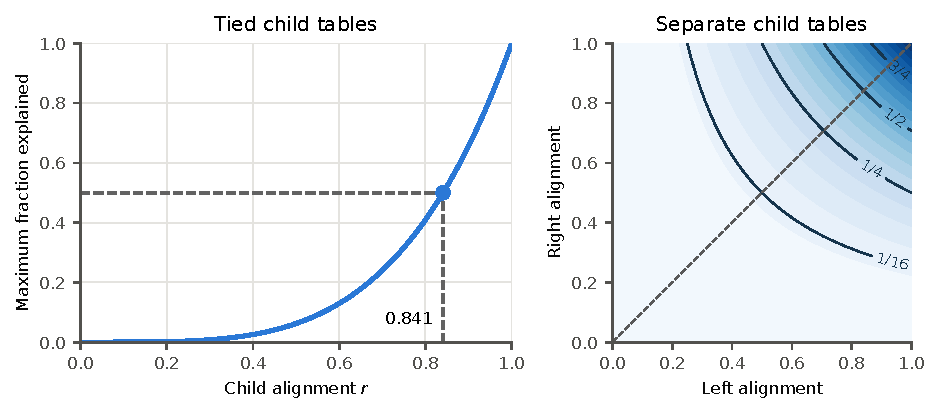
\includegraphics[width=.85\linewidth]{../../studies/rhm/child_feature_enabling/figures/frozen-root.pdf}
\caption{The best bilinear root explains $r_L^2r_R^2$ of the interaction variance. Each contour holds that fraction fixed. The dashed diagonal in the right panel recovers the tied curve on the left. Half the variance requires $r\ge 2^{-1/4}$ in the tied model, and the same product threshold constrains the two alignments in the untied model. Both panels show formulas, with no simulation data.}
\end{figure}
\section{What the children make available to a categorical root}
\label{sec:categorical-root}

Fix a binary RHM grammar of depth four and a TTN whose tree agrees with the
grammar. The root label is uniform on the $n$ classes. Each grammar symbol
chooses one of its $m$ ordered productions uniformly, independently of the
choices below it. Write $H_L,H_R\in\mathbb R^r$ for the representations
of the two eight-token subtrees and $Z=H_L\otimes H_R\in\mathbb R^{r^2}$
for their ordered product. In the repository's \texttt{TreeTN}, the root
maps this product directly to logits $CZ$, with $C\in\mathbb R^{n\times
r^2}$ and no bias. All formulas below apply to any fixed choice of the
lower cores, including a snapshot of jointly trained weights. For time
evolution with $Z$ fixed, the optimizer specified below is population
gradient flow. The repository trains with minibatch Adam.

\subsection{The population gradient of the actual classifier}

Let $e_Y$ denote the one-hot root label, let $p=\mathbf{1}/n$, and set
$D_j=\mathbb E[Z\mid Y=j]$ and $\bar D=\mathbb E Z$.
For cross-entropy, differentiating the log partition function gives
\begin{align}
 {\cal L}_{\rm CE}(C)
 &=\mathbb E\biggl[\log\sum_j e^{(CZ)_j} -(CZ)_Y\biggr],\\
 -\nabla_C{\cal L}_{\rm CE}(C)
 &=\mathbb E\big[(e_Y-\operatorname{softmax}(CZ))Z^\top\big].
 \label{eq:cat-full-gradient}
\end{align}
Resetting the root to zero makes its prediction $p$ for every tree. Its
initial descent direction $B$ therefore has rows
\begin{equation}
 B=\mathbb E[(e_Y-p)Z^\top],\qquad
 B_{j,:}=\frac{1}{n}(D_j-\bar D)^\top .
 \label{eq:cat-zero-gradient}
\end{equation}
If $B=0$, convexity of cross-entropy in the root weights makes $C=0$ a
global minimizer with loss $\log n$ on these frozen children. If $B\ne0$,
moving the root to $\eta B$ improves the loss by
$\eta\|B\|_F^2+O(\eta^2)$ for small $\eta>0$. Thus $B$ decides
\emph{exactly} whether a bilinear root can improve population
cross-entropy over the uniform predictor. This test compares full
matrices. One vanishing row or one vanishing root contrast establishes
only zero initial drive along that direction.

For a centered class contrast $c\in\mathbb R^n$ with $\sum_j c_j=0$,
write $R_j(u,v)=\Pr(U=u,V=v\mid Y=j)$ for the root rule probabilities
and $K_c(u,v)=n^{-1}\sum_j c_jR_j(u,v)$ for the signed rule table.
Let $M_L,M_R$ have columns $\mathbb E[H_L\mid U=u]$ and
$\mathbb E[H_R\mid V=v]$, respectively. Given the child symbols
$(u,v)$, the two subtrees expand independently. Averaging first over the
descendants and then over the root production gives
\begin{equation}
 \mathbb E[c_YH_LH_R^\top]
 =\sum_{u,v}K_c(u,v)\,M_L(:,u)M_R(:,v)^\top
 =M_LK_c M_R^\top .
 \label{eq:cat-contrast}
\end{equation}
Flattening this matrix gives $c^\top B$ in the order used to define $Z$.
For a singular term $\sigma a b^\top$ of $K_c$, its contribution is
$\sigma(M_La)(M_Rb)^\top$. A child that annihilates its side of this term
removes it from the drive. Other terms can survive or cancel in the sum.
When $K_c$ has zero row and column sums, collapsing either child's
conditional means to one common vector erases the entire contrast from
the initial drive. A generic grammar need not have these vanishing
marginals. For instance, a legal root table can encode the root class in
the left symbol alone, in which case even a constant nonzero right bond
can suffice.

\subsection{Exact moments without enumerating the leaf strings}

At each node $i$ with grammar symbol $s$ define
$\mu_i(s)=\mathbb E[H_i\mid s]$ and
$S_i(s)=\mathbb E[H_i H_i^\top\mid s]$. Use the tensor convention
$(x\otimes y)_{ab}=x_a y_b$. At leaf $i$, whose embedding of $s$ is
$h_i(s)$, the initial values are $h_i(s)$ and $h_i(s)h_i(s)^\top$.
At an internal node write the flattened core as $W_i$, so
$H_i=W_i(H_{iL}\otimes H_{iR})$. If the $k$th legal production of $s$
is $(u_k,v_k)$, conditional independence gives
\begin{align}
 d_i(s)&=\frac1m\sum_{k=1}^m \mu_{iL}(u_k)\otimes\mu_{iR}(v_k),\\
 F_i(s)&=\frac1m\sum_{k=1}^m S_{iL}(u_k)\otimes S_{iR}(v_k),\\
 \mu_i(s)&=W_i d_i(s),\qquad S_i(s)=W_i F_i(s)W_i^\top .
 \label{eq:cat-moments}
\end{align}
The second line uses $(x\otimes y)(x\otimes y)^\top
=(xx^\top)\otimes(yy^\top)$ before taking the conditional expectation.
At the root, stop before multiplying by its core. Then $D_j=d_{\rm
root}(j)$ and $F=n^{-1}\sum_j F_{\rm root}(j)=\mathbb E[ZZ^\top]$.
These contractions average only legal productions, with their true
probabilities. They apply to level-tied and untied weights because the
conditioning fixes the weights. A TTN that permutes leaves across
grammar subtrees requires a different contraction.

For any matrix perturbation $E$ of the root, the Hessian at zero obeys
\begin{equation}
 \nabla^2 {\cal L}_{\rm CE}(0)[E]
 =(\operatorname{diag}p-pp^\top)E F .
\end{equation}
This follows by differentiating the softmax in
\eqref{eq:cat-full-gradient}. At a nonzero root the softmax Jacobian
depends on the particular tree and stays inside the expectation. Thus
the two moments determine the exact initial gradient and curvature.
Evaluating the full nonlinear gradient at a trained root generally
requires more of the distribution of $Z$.

\subsection{Fitting a root above frozen children}

To quantify what a frozen representation can predict at arbitrary root
weights, take a scalar target $y=c_Y$ and fit the same bias-free root
with population squared error. With $b=\mathbb E[Zy]$, expansion gives
\begin{equation}
 2{\cal L}_2(w)=\mathbb E[y^2]-2w^\top b+w^\top Fw .
\end{equation}
For $v\in\ker F$, $\mathbb E[(v^\top Z)^2]=0$, so $v^\top b=0$ as well.
Consequently $b$ lies in the range of $F$, $w_*=F^\dagger b$ is a
minimizer, and completing the square gives
\begin{equation}
 2{\cal L}_2(w)=\mathbb E[y^2]-b^\top F^\dagger b
                  +(w-w_*)^\top F(w-w_*) .
 \label{eq:cat-oracle}
\end{equation}
Here $F^\dagger$ is the Moore--Penrose pseudoinverse. For a nonzero contrast,
the fraction of its variance explained by the root is
$b^\top F^\dagger b/\mathbb E[y^2]$. It is invariant under any
invertible change of basis on either child bond. Indeed, such a change preserves the set of
scalar predictions $w^\top Z$ after reparametrizing $w$. The Euclidean
gradient and its speed depend on that parametrization.

For a fresh root $w(0)=0$, gradient flow obeys $\dot w=b-Fw$.
Diagonalize $F$ with orthonormal eigenvectors $v_k$ and positive
eigenvalues $\lambda_k$. Each component obeys
\begin{equation}
 v_k^\top w(t)=\frac{v_k^\top b}{\lambda_k}
       (1-e^{-\lambda_k t}),\qquad
 {\cal L}_2(w(t))-{\cal L}_2(w_*)
 =\frac12\sum_{\lambda_k>0}
 \frac{(v_k^\top b)^2}{\lambda_k}e^{-2\lambda_k t}.
\end{equation}
A nonzero component reaches half its final amplitude at
$\log 2/\lambda_k$. This separates a better attainable fit from a
shorter learning time in fixed coordinates. These are regression
half-times for freshly trained roots at different lower-core snapshots.
They do not give hitting times for the jointly trained categorical model.

\paragraph{Why a shared factor does not imply a lag.}
In the symmetric two-mode model $f_i=a b_i z_i$ with equal targets and
equal private initial conditions, exchanging indices $1,2$ leaves the
loss and initialization invariant. Uniqueness of gradient flow then
implies $b_1(t)=b_2(t)$ and $z_1(t)=z_2(t)$, so the two modes hit every
common threshold together despite sharing the trainable factor $a$.
More generally a change $H_L\mapsto \alpha H_L$, $C\mapsto C/\alpha$
preserves every categorical prediction while changing the apparent
size of the child feature. A quantitative time-gap theorem must specify
a distribution, a target contrast, the initialization, and the optimizer's
metric, as well as the intervention that tests necessity.

\section{Which gradient reaches an interior core?}
\label{sec:interior}
The root calculation extends to every internal core of an aligned multilinear
student under squared loss. An interior core receives information from both
the child subtrees and the part of the network that uses its output.
Conditioning on its grammar symbol separates those two contributions.

At position $i$ put $z_i=h_{iL}\otimes h_{iR}$, $h_i=W_i z_i$,
and write the student output as $f=A_i h_i$. Here $A_i$ maps changes
at this occurrence of the bond to the logits, holding the other subtree
activations fixed. It depends only on observations outside the subtree at $i$
when parameters are fixed. Denote the grammar symbol by $S_i=s$,
with probability $p_i(s)>0$, and define
\[
 d_i(s)=\mathbb E[z_i\mid s],\quad F_i(s)=\mathbb E[z_i z_i^\top\mid s],
 \quad m_i(s)=\mathbb E[A_i^\top e_Y\mid s],\quad
 N_i(s)=\mathbb E[A_i^\top A_i\mid s].
\]
Then the negative gradient from this occurrence is exactly
\begin{equation}
 -\nabla_{W_i}\mathcal L_2
 =\sum_s p_i(s)\left[m_i(s)d_i(s)^\top-N_i(s)W_iF_i(s)\right].
 \label{eq:interior}
\end{equation}
Indeed the sample gradient is
$A_i^\top(e_Y-A_i W_i z_i)z_i^\top$ with the descent sign.
Conditioned on $s$, the outside variables $(A_i,Y)$ are independent of
the draws that expand this subtree. Taking the expectation of each product
yields~\eqref{eq:interior}. If several occurrences share a table, sum all
their partial derivatives. Freezing other occurrences while evaluating
each partial derivative is precisely the chain rule for tying.

The two inward messages $d_i,F_i$ are already available in
Section~\ref{sec:categorical-root}. The two outward messages also have an
exact recursion. At the root use $A=I$, $m(y)=e_y$, $N(y)=I$.
For a left descent from parent $i$, let $B_i(v)$ denote the matrix
mapping $u$ to $W_i(u\otimes v)$. For fixed sibling activation $h_R$,
$A_L=A_i B_i(h_R)$. The probability that the parent is $a$ and the
sibling symbol is $c$, conditional on the left symbol $b$, is
\[
 \omega(a,c\mid b)=\frac{p_i(a)G_{\ell(i)}(a,b,c)}
 {\sum_{a',c'}p_i(a')G_{\ell(i)}(a',b,c')}.
\]
Unused symbols can be skipped. Writing $\mu_R(c)=\mathbb E[h_R\mid c]$,
independence of the outer context and the parent production conditional
on $a$, and independence of the sibling expansion given $c$, give
\begin{align*}
 m_L(b)&=\sum_{a,c}\omega(a,c\mid b)\,
        B_i(\mu_R(c))^\top m_i(a),\\
 N_L(b)&=\sum_{a,c}\omega(a,c\mid b)\,
 \mathbb E[B_i(h_R)^\top N_i(a) B_i(h_R)\mid c].
\end{align*}
The last integrand is quadratic in $h_R$, so its conditional second
moment suffices. Exchanging child roles gives the corresponding right
messages. At the root, \eqref{eq:interior} reduces to $D/n-CF$ with the
notation of \eqref{eq:full-square}. This argument needs neither independent
child symbols marginally nor a diagonal student. It gives all population
gradients without first selecting a set of teacher modes. A particular
update can still cancel after summing over symbols or tied positions.
For softmax loss the predicted-probability term depends on the entire
logit vector, so this squared-loss factorization no longer follows.

\section{A local test for enabling in the softmax TTN}
\label{sec:escape}
The two-head example singles out a direction in a lower representation.
For the categorical loss we can also decide exactly whether permitting
a specified block of lower parameters to move creates a descending
quadratic direction at the uniform predictor. This local result applies
to the architecture in the training code. It requires a stationary point
of a particular kind. A generic checkpoint need not satisfy the premise.

Write $Z_\theta$ for the product of the two child features and
$B(\theta)=\mathbb E[(e_Y-p)Z_\theta^\top]$.
Consider a point $(C,\theta)=(0,\theta_0)$ with $B(\theta_0)=0$.
The joint gradient vanishes there: resetting the root erases all
first derivatives with respect to the children, and the root gradient
also vanishes by hypothesis. Work in the softmax gauge
$\mathbf1^\top C=0$. Let $v$ be a parameter perturbation supported on
the allowed child block and $E$ a centered perturbation of the root.
Set $Jv=\mathrm d B(\theta_0)[v]$ and $F_0=\mathbb E[Z_0Z_0^\top]$.
The Hessian quadratic form in direction $(E,v)$ is
\begin{equation}
 Q(E,v)=n^{-1}\operatorname{tr}(E F_0 E^\top)-2\langle E,Jv\rangle_F .
 \label{eq:escape-hessian}
\end{equation}
To derive it, expand $C=tE,\theta=\theta_0+tv$. The linear term
in $C$ is $-t\langle E,B(\theta_0+tv)\rangle_F$. The quadratic softmax
term at $C=0$ uses the class covariance $I/n-\mathbf1\mathbf1^\top/n^2$.
All derivatives exist because the grammar has finite support and the
TTN is polynomial before softmax. The child-only Hessian is zero since
$\mathcal L(0,\theta)=\log n$ identically.

\begin{proposition}
At such a point the joint Hessian restricted to the chosen parameters
has a negative eigenvalue if and only if $J$ is nonzero on the allowed
child directions.
\end{proposition}
\begin{proof}
If $Jv\ne0$, take $E=\alpha Jv$, with $\alpha>0$ sufficiently small.
The negative term in \eqref{eq:escape-hessian} is linear in $\alpha$ and
the nonnegative term is quadratic, so $Q(E,v)<0$. If $J=0$ the form is
positive semidefinite. This argument also covers singular $F_0$.
\end{proof}

The grammar identifies the source of $J$. For each contrast $c$,
differentiate~\eqref{eq:cat-contrast}:
\[
 \mathrm d (M_LK_cM_R^\top)[v]
 =(\mathrm dM_L[v])K_cM_R^\top
  +M_LK_c(\mathrm dM_R[v])^\top.
\]
For a tied parameter both contributions must be added before testing
for a nonzero direction. For example, if $K_c=uv^\top$ and
$M_Lu=M_Rv=0$, both terms vanish. If just the right side carries $v$,
a perturbation giving $\mathrm dM_L[v_{\rm par}]u\ne0$ suffices.
A different contrast with a one-child marginal can produce a negative
eigenvalue at the very same representation. The test identifies which
parameter changes have first-order access to the label. A nonzero
derivative for another contrast does not by itself show that its
unstable trajectory moves in the direction the interaction needs.

\paragraph{What happens when the first derivative vanishes?}
There is an exact leading-order law for the best local root fit.
Assume $F_0$ is positive definite on the fixed feature coordinates being
fit. For a smooth child path $\theta(t)$ through $\theta_0$ such that
$B(\theta(t))=t^d B_d+o(t^d)$ with $B_d\ne0$,
\begin{equation}
 \min_C \mathcal L_{\rm CE}(C,\theta(t))
 =\log n-\frac{n}{2}t^{2d}
 \operatorname{tr}(B_d F_0^{-1} B_d^\top)+o(t^{2d}).
 \label{eq:escape-profile}
\end{equation}
Indeed on centered rows the derivative of the root gradient at zero is
$E\mapsto EF_0/n$, an invertible operator. For small $t$ the implicit
function theorem yields a stationary root $C_*(t)$. Convexity in the
root makes this a global minimizer. More explicitly the root gradient
is $-B+C F(t)/n+O(\|C\|^2)$ with a uniform Taylor bound near the
point. Uniform invertibility implies $C_*=O(\|B\|)$ and then
$C_*=n B F_0^{-1}+o(\|B\|)$. Substitution into the quadratic expansion
of the loss gives~\eqref{eq:escape-profile}.
A product of two missing child contrasts therefore yields quartic
improvement along a path where both turn on linearly, provided no lower
order signal survives in the fitted logits. A one-child signal can give
quadratic improvement. Constant null directions can be removed first.
An emerging feature direction can change the rank of $F$ and invalidate
this inverse expansion. The Hessian criterion itself
(\eqref{eq:escape-hessian}, with a negative eigenvalue as above) does
not need invertibility. Equation~\eqref{eq:escape-profile} describes a
root refitted along a prescribed path. Converting its order to a joint-flow
escape time requires a dynamical argument such as Section~\ref{sec:parity-toy}.

\paragraph{An exact rank-changing obstruction.}
Consider two classes $Y=\pm1$ uniformly and one scalar feature $Z_t=tY$.
At $t=0$ every root predicts uniform class probabilities. For every $t>0$
the one-dimensional feature separates the classes and the infimum of
cross-entropy over unconstrained roots is zero: logits $(kZ_t,-kZ_t)$
in the matching class order have loss $\log(1+e^{-2kt})$.
Here $F(t)=t^2$ loses rank at the base point. Infinitesimal signal
therefore permits an order-one improvement if root weights may grow
without bound. The distinction between an optimally refitted root and
the finite time required by a specified optimizer is essential.

For a concrete nonsingular comparison, let $H,N$ be independent uniform
signs on one subtree and take its feature to be $h_t=N+tH$ on a prescribed
path. For a binary root contrast $Y=H$ with a single feature $Z=h_t$,
$\mathbb E[YZ]=t$ and $\mathbb E[Z^2]=1+t^2$. For the pure interaction
on two independent copies, use $Y=H_LH_R$ and $Z=h_{t,L}h_{t,R}$.
Now $\mathbb E[YZ]=t^2$ and $\mathbb E[Z^2]=(1+t^2)^2$.
For logits $(wZ,-wZ)$ and the matching sign convention the binary loss is
$\mathbb E\log(2\cosh wZ)-w\mathbb E[YZ]$.
Its curvature at $w=0,t=0$ is one in both cases. Thus the optimal CE
improvement along this path is $t^2/2+o(t^2)$ with the one-child target
and $t^4/2+o(t^4)$ with the interaction. This comparison specifies both
the directions the children develop and the observable whose change
is measured.

\section{Which root contrasts require an interaction in the three training grammars?}
\label{sec:rule-audit}

The parity example has a root contrast whose conditional mean given either
child alone is zero. We can check that property exactly in the three
quenched grammars used in the root-classification experiments. For each of
the \(n=16\) root symbols, enumerate its \(m=4\) legal top productions. A
row \(e\) records a root label \(j_e\) and an ordered child pair
\((u_e,v_e)\). Under the uniform root and uniform production law, the
\(nm=64\) rows have equal probability. The calculation uses the actual
hidden child symbols and asks what information is available even with
perfect access to them.

Let \(E\) be the \(64\times16\) one-hot label matrix and let \(D\) be the
\(64\times32\) matrix whose row has a one in left column \(u_e\) and
another in right column \(16+v_e\), using zero-based indices. A root contrast
\(c\in\mathbb R^{16}\) assigns the value \(y_e=(Ec)_e=c_{j_e}\) to
each row. Every prediction of the form \(f(u_e)+g(v_e)\) lies in
\(\operatorname{col}D\), and every vector in that column space has such a
representation. Centered root contrasts satisfy \(\sum_j c_j=0\).

\paragraph{Two dimension counts.}
The vector \(D^\top Ec\) contains the sums of \(y_e\) within each left
symbol and within each right symbol. On a symbol of positive probability,
its sum vanishes exactly when its conditional mean vanishes. Let us call
a contrast \emph{purely interactive} when both sets of marginal signals
vanish. The kernel of \(D^\top E\) consists of exactly those contrasts.
They are already centered because constants belong to \(\operatorname{col}D\).
At the opposite extreme \(Ec\) itself may be additive on the legal
productions. Since \(E^\top E=m I\), the map from contrasts to edge
values is injective. The dimension formula for the intersection of two
subspaces gives
\begin{align}
 d_{\rm pure} &= n-\operatorname{rank}(D^\top E),\\
 d_{\rm additive,centered}
 &= n+\operatorname{rank}D-\operatorname{rank}[D\ E]-1 .
\end{align}
The last subtraction removes the shared constant. Both ranks are computed
over the rationals from integer matrices.

\paragraph{How much can an additive predictor explain?}
Let \(P_D=DD^\dagger\), the orthogonal projection onto additive functions
on these rows. For a nonzero centered contrast, the fraction of its
population variance explained by its best additive predictor is
\[
 \eta(c)=\frac{\|P_D Ec\|^2}{\|Ec\|^2}.
\]
Indeed, the uniform row weights cancel in the ratio, and the projection
minimizes the squared residual. If \(H\) has orthonormal columns spanning
\(\mathbf 1^\perp\) in label space, then \(Q=EH/\sqrt m\) has orthonormal
columns in row space. The minimum and maximum of \(\eta\) are the extreme
eigenvalues of \(Q^\top P_DQ=(P_DQ)^\top(P_DQ)\). These fractions allow
both children's separate contributions to enter in the same additive fit,
including any correlations between the two child symbols.

\begin{center}
\begin{tabular}{c|ccc|cc}
Seed & \(\operatorname{rank}D\) & \(\operatorname{rank}(D^\top E)\)
& \(\operatorname{rank}[D\ E]\) & \(\min\eta\) & \(\max\eta\)\\ \hline
0 & 30 & 16 & 45 & 0.063505 & 0.927720\\
1 & 31 & 16 & 46 & 0.108409 & 0.821812\\
2 & 31 & 16 & 46 & 0.063091 & 0.909308
\end{tabular}
\end{center}

For each seed both dimension counts are zero. Every nonzero centered root
contrast has some marginal signal, so a pure parity contrast cannot be
selected from the sixteen label values in these tables. Every such contrast
also retains a nonzero residual after its best additive fit. For seed 0,
the least additive direction retains \(93.65\%\) of its variance in that
residual. That makes it a candidate for studying how learning the children
changes the root's access to information about their joint state.
Residualizing \(Ec\) against \(D\) would produce an exactly pure edge
target, but its values can differ across productions of the same root.
That intervention would change the prediction task.

To reproduce the calculation from the repository root, run
\begin{quote}
\small\ttfamily python3 -m studies.rhm.child\_feature\_enabling.grammar\_audit
\end{quote}
It enumerates the root tables from \texttt{studies.rhm.common.GRAMMAR}
with seeds 0, 1, and 2. The accompanying JSON records the tables, all
fifteen eigenvalues per seed, the exact ranks, the grammar settings, and
hashes of the grammar source files. The code checks the projection spectrum
against an independent principal-angle calculation. A planted binary parity
table and a table in which the root equals the left child check the pure
and additive endpoints, respectively.

\begin{figure}[htbp]\centering
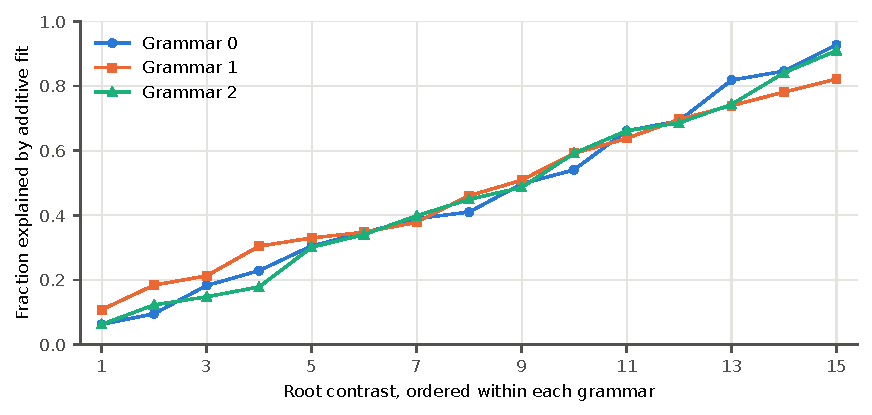
\includegraphics[width=.74\linewidth]{../../studies/rhm/child_feature_enabling/figures/grammar-spectra.pdf}
\caption{Additive predictability of fifteen orthogonal centered root contrasts per fixed grammar, computed over its 64 equiprobable top rules. The sorted eigenvalues belong to a different contrast basis for each grammar. A zero eigenvalue would give an exactly pure interaction, while an eigenvalue of one would identify a fully additive label contrast.}
\end{figure}
\section{A shared lower factor changes the gap between learning times}
\label{sec:shared-gap}

Consider the aligned model from November 18. Two orthogonal teacher components
of strengths \(s_1>s_2>0\) use the same unit feature on the left branch of a
tree. The student assigns the shared feature an amplitude \(a\). On the right
branch and at the root, component \(k\) has private amplitudes \(b_k,r_k\).
Under squared loss on whitened tensor-product inputs, the two coefficients
\(c_k=a r_k b_k\) have loss
\(\mathcal L=\tfrac12\sum_{k=1}^2(s_k-c_k)^2\). All times below refer to
Euclidean gradient flow with unit learning rate on the individual factors.
We initialize \(r_k=b_k=\delta\) and \(a=\sqrt{2}\delta\).
The alignment and positive balanced initialization are assumptions.

\begin{theorem}[Learning-time gap for one shared factor]
\label{thm:shared-gap}
Let \(T_k(q)=\inf\{t:c_k(t)\ge q s_k\}\) for a fixed \(0<q<1\). At fixed
\(s_1>s_2>0\), as \(\delta\downarrow0\),
\begin{equation}
 T_2(q)-T_1(q)=
 s_1^{-1/3}\left(\frac{1}{s_2}-\frac{1}{s_1}\right)
 \log(1/\delta)+O(1).
 \label{eq:shared-gap}
\end{equation}
Both \(T_k(q)\) are of order \(\delta^{-1}\).
\end{theorem}

\begin{proof}
Write \(\epsilon_k=s_k-c_k\). The three derivatives are
\[
 \dot a=\sum_k r_k b_k\epsilon_k,\qquad
 \dot r_k=a b_k\epsilon_k,\qquad \dot b_k=a r_k\epsilon_k .
\]
Thus \(r_k^2-b_k^2\) and \(a^2-\sum_k r_k^2\) are constant, both zero
at initialization. Put \(p_k=r_k^2=b_k^2\), so \(a=\sqrt{p_1+p_2}\),
\(c_k=ap_k\), and \(a^3=c_1+c_2\). In the time variable
\(u(t)=\int_0^t a(t')\,dt'\), the equations become
\[
 p_k'=2p_k(s_k-ap_k),\qquad
 (1/p_k)'=-2s_k/p_k+2a.
\]
Integration gives an exact formula and two bounds,
\begin{align}
 \frac{1}{p_k(u)} &=
 \delta^{-2}e^{-2s_k u}
 +2\int_0^u a(v)e^{-2s_k(u-v)}\,dv, \label{eq:shared-recip}\\
 \frac{1}{\delta^{-2}e^{-2s_ku}+A/s_k}
 &\le p_k(u)\le\delta^2 e^{2s_ku}. \label{eq:shared-bounds}
\end{align}
Here \(A\) is independent of small \(\delta\). Indeed, loss decreases, so
each \(c_k\) is bounded and \(a^3=c_1+c_2\) gives \(a\le A\). The lower
bound on \(p_k\) then keeps \(a\) positive for each \(\delta>0\), and
\(u\) runs from zero to infinity.

\emph{Where are the two crossings in \(u\)?}
Set \(L=\log(1/\delta)\) and \(U_k=L/s_k\).
The upper bound on \(p_k\) gives \(c_k\le A\exp(2s_k(u-U_k))\).
The lower bound gives \(p_k\ge m_k=(1+A/s_k)^{-1}\) for \(u\ge U_k\).
We claim the first crossing of \(q s_k\) occurs at \(u=U_k+O(1)\).
The upper bound on \(c_k\) prevents either crossing earlier than
\(U_k-O(1)\). Until \(c_1\ge q s_1\), the exact equation gives
\(p_1'\ge 2(1-q)s_1p_1\). Since \(m_1\le p_1\le A^2\), this
forces a crossing within a bounded time after \(U_1\). The same argument
with \(m_2,s_2\) proves the claim for component 2.

\emph{How much physical time separates the crossings?}
On \([U_1,U_2]\), the total integral of the weaker private amplitude is bounded,
\[
 \int_{U_1}^{U_2}p_2(u)\,du\le
 \int_{U_1}^{U_2}\exp(2s_2(u-U_2))\,du\le \frac{1}{2s_2}.
\]
With \(p_2=0\) the stable positive value of \(p_1\) is \(p_*=s_1^{2/3}\).
For \(h=\log(p_1/p_*)\) the exact equation is
\[
 h'=-2s_1(e^{3h/2}-1)
       -2p_1\bigl(\sqrt{p_1+p_2}-\sqrt{p_1}\bigr).
\]
The second term is bounded in magnitude by \(C p_2\), since \(p_1\) lies
in \([m_1,A^2]\). On this same compact interval of \(p_1\), the first term
is \(-\lambda(u)h\) with
\(\lambda(u)=2s_1(e^{3h/2}-1)/h\) bounded below by a positive constant
\(\lambda_0\), using the continuous value at zero. The integrating factor
therefore bounds
\[
 |h(u)|\le |h(U_1)|e^{-\lambda_0(u-U_1)}
       +C\int_{U_1}^{u}e^{-\lambda_0(u-v)}p_2(v)\,dv .
\]
Integrating once more gives \(\int_{U_1}^{U_2}|h|\,du=O(1)\).
The function \(1/\sqrt{p_*e^h+p_2}\) has bounded first derivatives on
this range, so
\[
 \int_{U_1}^{U_2}\left|\frac1a-s_1^{-1/3}\right|du=O(1).
\]
A bounded displacement of either endpoint changes physical time by \(O(1)\),
since~\eqref{eq:shared-bounds} bounds \(a\) below around both endpoints.
Thus integrating \(dt=du/a\) proves~\eqref{eq:shared-gap}.

Finally, on \([0,U_1]\), the lower bound on \(p_1\) gives
\(1/a\le\delta^{-1}e^{-s_1u}+\sqrt{A/s_1}\). On \([0,1]\) both
\(p_k\le \delta^2e^{2s_k}\), which gives \(1/a\ge C/\delta\).
Integrating yields \(t(U_1)=\Theta(\delta^{-1})\), as claimed.
\end{proof}

The strong mode's private factor grows first. Near its crossing, the weak
private factor still has \(p_2=\Theta(\delta^{2(1-s_2/s_1)})\)
by~\eqref{eq:shared-bounds}. For most of the intervening time the common
factor has \(a\simeq s_1^{1/3}\), in the integrated sense proved above.
This lets the weak private factors grow exponentially at an order-one rate.
If each coefficient instead owns three independent positive balanced factors
of common amplitude \(x_k\), then \(\dot x_k=x_k^2(s_k-x_k^3)\).
Its crossing time is
\[
 \int_\delta^{(q s_k)^{1/3}}\frac{dx}{x^2(s_k-x^3)}
 =\frac{1}{s_k\delta}+O(1),
\]
since subtracting \(1/(s_kx^2)\) leaves an integrand of order \(x\) at
zero. The independent gap is of order \(1/\delta\). In the shared model
the gap diverges logarithmically, even though \(T_2/T_1\to1\).

\paragraph{What requires learning the shared feature?}
Freeze just \(a\) at \(a_0=\sqrt2\delta\) from initialization, keeping
the root and right branch trainable. The weak coefficient now obeys
\(\dot c_2=2a_0 c_2(s_2-c_2)\) and has \(c_2(0)=a_0\delta^2\).
Separating variables gives the exact crossing time
\begin{equation}
 T_2^{\rm frozen}(q)=\frac{1}{2a_0s_2}
 \log\!\left[\frac{q}{1-q}
       \left(\frac{s_2}{a_0\delta^2}-1\right)\right]
 \sim \frac{3\log(1/\delta)}{2\sqrt2\,s_2\delta}.
 \label{eq:shared-frozen}
\end{equation}
Thus movement of the lower factor is necessary to achieve the
\(\Theta(\delta^{-1})\) hitting time under this intervention. The positive
frozen model still fits in the limit of long training. Removing the strong
teacher signal is a different intervention, since the weak signal can itself
train \(a\).

\subsection{How the number of private factors sets the rate}
\label{sec:private-degree}
A single aligned contraction can contain \(m\) trainable private factors
with product \(x_1\cdots x_m\). Let \(g(t)>0\) denote the product of its
shared factors, and suppose the private parameters enter a squared loss only
through \(c=g\prod_j x_j\) with target \(s>0\). Equal positive initialization
\(x_j(0)=\delta\) is invariant under Euclidean gradient flow, so all
private factors equal \(x(t)\). Each factor receives the derivative of
one copy of the product, hence
\[
 \dot x=g(t)x^{m-1}\bigl(s-g(t)x^m\bigr).
\]
Up to the first fixed-fraction crossing \(c=q s\), integration yields
\[
 \int_\delta^{x(t)} z^{1-m}\,dz
   =\int_0^t g(v)(s-c(v))\,dv
   \ \in\
 \left[(1-q)s\int_0^t g(v)\,dv,\;
                   s\int_0^t g(v)\,dv\right].
\]
The accumulated product of the shared factors therefore controls the private
amplitude. One must determine how \(g(t)\) evolves to extract a physical
time gap.

For a fixed value \(g>0\), integration to \(x_q=(qs/g)^{1/m}\) gives
\[
 T(q;g)=\frac{1}{g s}
        \int_\delta^{x_q}\frac{x^{1-m}}{1-gx^m/s}\,dx .
\]
For fixed \(s,q,g\), the time is finite as \(\delta\downarrow0\) for \(m=1\),
logarithmic for \(m=2\), and polynomial for \(m>2\). More precisely,
\[
 T(q;g)=
 \begin{cases}
  g^{-2}\log(1/(1-q))+o(1), &m=1,\\
  (g s)^{-1}\log(1/\delta)+O(1), &m=2,\\
  \delta^{-(m-2)}/[g s(m-2)]+O(1), &m>2 .
 \end{cases}
\]
For the first line solve \(\dot c=g^2(s-c)\) directly. In the other two
lines subtract \(x^{1-m}\) from the integrand. The remainder is
\((g/s)x/(1-gx^m/s)\), integrable down to zero. Thus even an order-one
shared feature leaves a polynomial escape time if a dormant mode still
needs three or more small private factors. A TTN with multiple contraction
paths or mixed target directions requires a separate justification for this
scalar reduction.

\end{document}
